% !TEX root = ../Hamiltonian_of_mean_force.tex
\section{Numerical Validation}
\label{sec:numerical_results}

The exact solution of Sec.~\ref{sec:qubit_direct_response_v5} depends on the
bath only through the kernel evaluated at three frequencies,
$\omega \in \{0, \pm\omega_q\}$.
To test it we compare against Exact Diagonalisation (ED) of a truncated
spin-boson model: the qubit is coupled to $N_\omega$ harmonic oscillators,
each represented with a per-mode Fock cutoff $n_{\max}$.
A key feature of this comparison is that the analytic kernel integrals
$\mathcal{K}(\omega) = \int_0^\infty d\nu\, J(\nu)\, \mathcal{F}(\nu,\omega,\beta)$
can be evaluated in two ways: using the full continuum spectral density
(the \emph{continuous analytic} branch) or restricted to the same $N_\omega$
discrete modes seen by ED (the \emph{discrete analytic} branch).
Distinguishing between these is essential for identifying the true origin 
of numerical discrepancies in the strong-coupling regime.

Figure~\ref{fig:ed_vs_analytic} shows the excited-state population $p_{11}$
as a function of coupling strength and inverse temperature, each for $N_\omega = 40$ modes. At weak coupling ($\chi \ll 1$) all three curves coincide.
However, as the system crosses into the strong-coupling regime ($\chi \gtrsim 1$),
the analytic predictions separate from the ED results. The key to interpreting this gap lies in the branching between the analytic solution using either the \emph a \emph{continuous} (dotted orange line) or \emph{discrete} (blue dashed line) spectral density. We see that as $\chi$ increases into the crossover region and beyond,
the discrete analytic result decouples from the ED curve and instead converges back to the continuous spectrum analytic solution, correctly converging to the
ultrastrong limit. This is a powerful result: it shows that the HMF
theory is exact even for small, discrete mode sets, and that a discrete 
bath is physically capable of reaching the ultrastrong limit.

The fact that ED (green solid) remains significantly higher than its own
infinite-cutoff analytic prediction is therefore not a failure of the theory,
nor even a finite-mode artifact. Rather, it is a \emph{representability bottleneck} in the dimension of those modes. In the ultrastrong limit, the coupled system seeks a displaced ground state (a polaron-like state) where each mode $k$ is displaced from vacuum by $\alpha_k \sim g_k/\omega_k$. Representing such a state faithfully requires
a level cutoff $n_{\max} \gtrsim |\alpha_k|^2$. When $\chi \gtrsim 1$, the
available Fock space in the ED simulation is insufficient to capture the
tails of these displaced oscillators. The system is "trapped" in a subspace
of artificially low occupation numbers, leading to over-estimated energies
and the persistent gap observed at large $\chi$.

\begin{figure}[t]
  \centering
  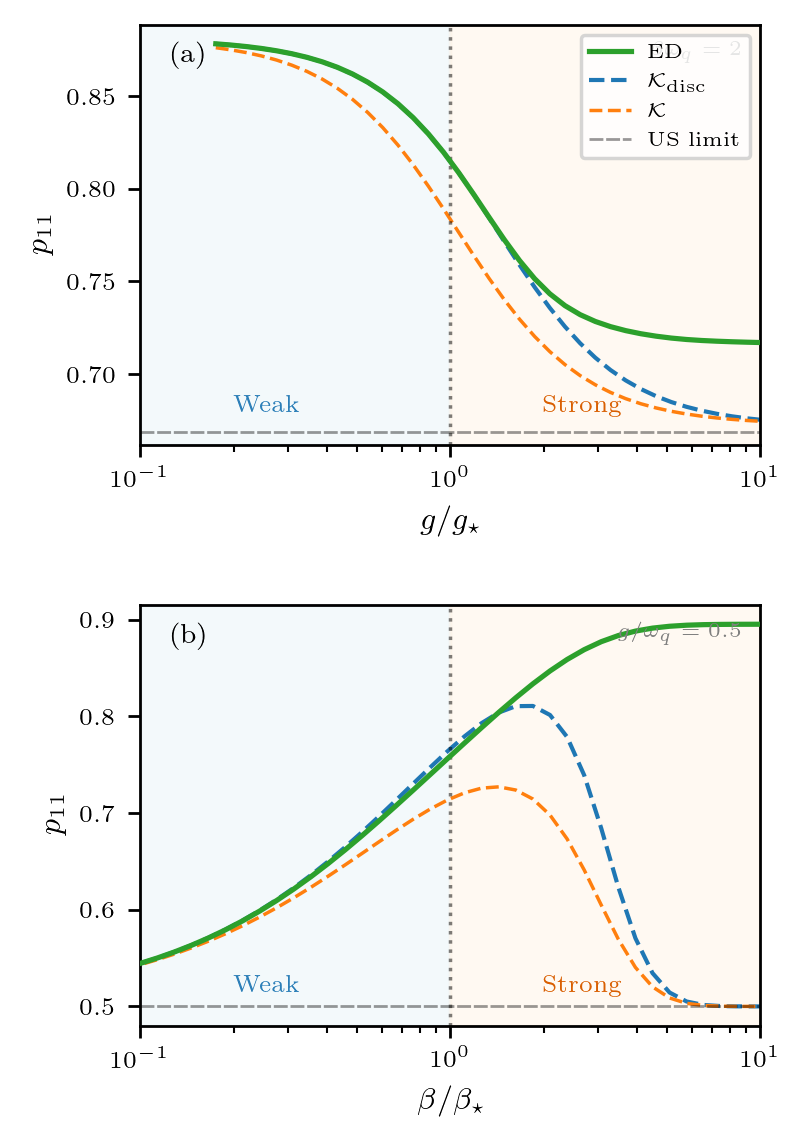
\includegraphics[width=0.48\textwidth]{../figures/hmf_fig2_ed_vs_analytic.png}
  \caption{Excited-state population $p_{11}$ across the $\chi$-crossover
    for $N_\omega=40$ modes.
    Green solid: ED.  Blue dashed: discrete analytic (same $N_\omega$ modes).
    Orange dotted: continuous analytic.
    Dashed horizontal lines mark the ultrastrong limit $p_\infty$.
    The discrete analytic correctly reaches the US limit, 
    matching the continuum. The gap left by ED (green) is a representability 
    failure: the fixed Fock cutoff cannot accommodate the mode displacements 
    required to reach the true HMF state.}
  \label{fig:ed_vs_analytic}
\end{figure}

The representability bottleneck implies that simulation accuracy should be 
highly sensitive to the choice of mode cutoffs as one enters the 
strong-coupling regime. Figure~\ref{fig:bandwidth_convergence} explores 
this by monitoring the cutoff sensitivity $\Delta p_{11}$
as a function of the spectral window bandwidth $B$ (in units of $\omega_q$).

The presence of a distinct peak in the sensitivity is a direct 
signature of the modes hitting the Fock boundary. As $\chi$ grows (lower 
temperatures), the requirement for mode displacements increases, pushing the 
available Fock space to its limit. This ``simulability crossover" occurs 
exactly where $\chi \sim 1$, providing a concrete numerical marker for the 
validity of the finite-dimension approximation to the reduced equilibrium state. 

In summary, the numerical results establish that the analytic HMF provides 
the correct physical target for both discrete and continuous baths. The 
deviations seen in simulation are not theoretical errors but markers of the 
intrinsic difficulty in representing the strongly-dressed open-system ground 
state within a finite Fock basis. The crossover parameter $\chi$ emerges as 
the universal controller of this simulability crossover, just as it 
governs the analytic structure of the state itself. It reveals that within the crossover regime, even the simplest systems contain rich nonlinearities in response to coupling and temperature, which cannot be efficiently accessed by standard numerical methods. More evidence - as if it were needed - of the fundamental importance of the exact strong coupling solution.

\begin{figure}[t]
  \centering
  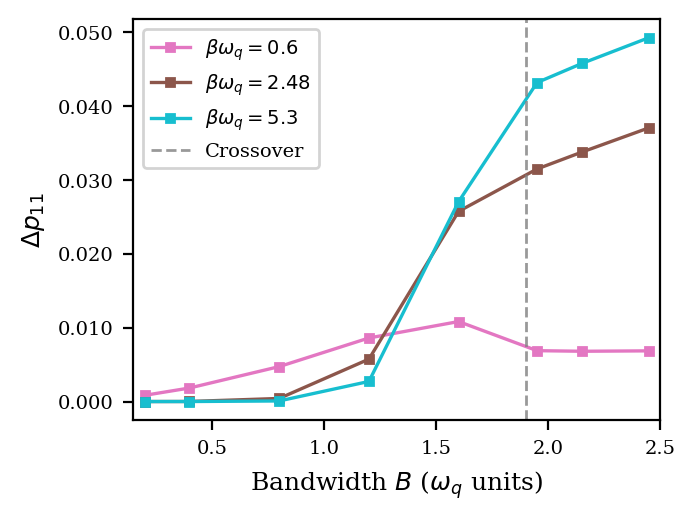
\includegraphics[width=0.48\textwidth]{../figures/hmf_fig3_bandwidth_convergence.png}
  \caption{Cutoff sensitivity $\Delta p_{11} \equiv |p_{11}(n_{\max}=4) - p_{11}(n_{\max}=6)|$
    as a function of spectral bandwidth $B$ (measured in units of $\omega_q$). 
    The vertical dashed line marks the crossover where mode occupation 
    requirements begin to exceed the available Fock space. The sensitivity 
    peaks sharply as the system enters the strong-coupling regime ($\chi \gtrsim 1$), 
    marking the onset of the representability bottleneck. Higher sensitivity 
    at lower temperatures reflects the increased mode-occupation required 
    to represent the displaced ultrastrong state.}
  \label{fig:bandwidth_convergence}
\end{figure}

